
\subsection{Probe A}
\subsubsection{Leitfähigkeit und Hall-Koeffizient}
%auswerteformeln und probendimensionen angeben

Leitfähigkeit und Hall-Koeffizient der Proben sind Temperaturabhängig.
Es gelten die folgenden Beziehungen:
$$R_H = \frac{U_{H} \cdot b}{ I \cdot B }$$
$$\sigma = \frac{l \cdot I}{b \cdot d \cdot U_{leit}}$$

wobei $l = 19 \text{mm}$, $b = 10 \text{mm}$ und $d = 1 \text{mm}$

\begin{figure}
\label{fig:R_H}
\centering
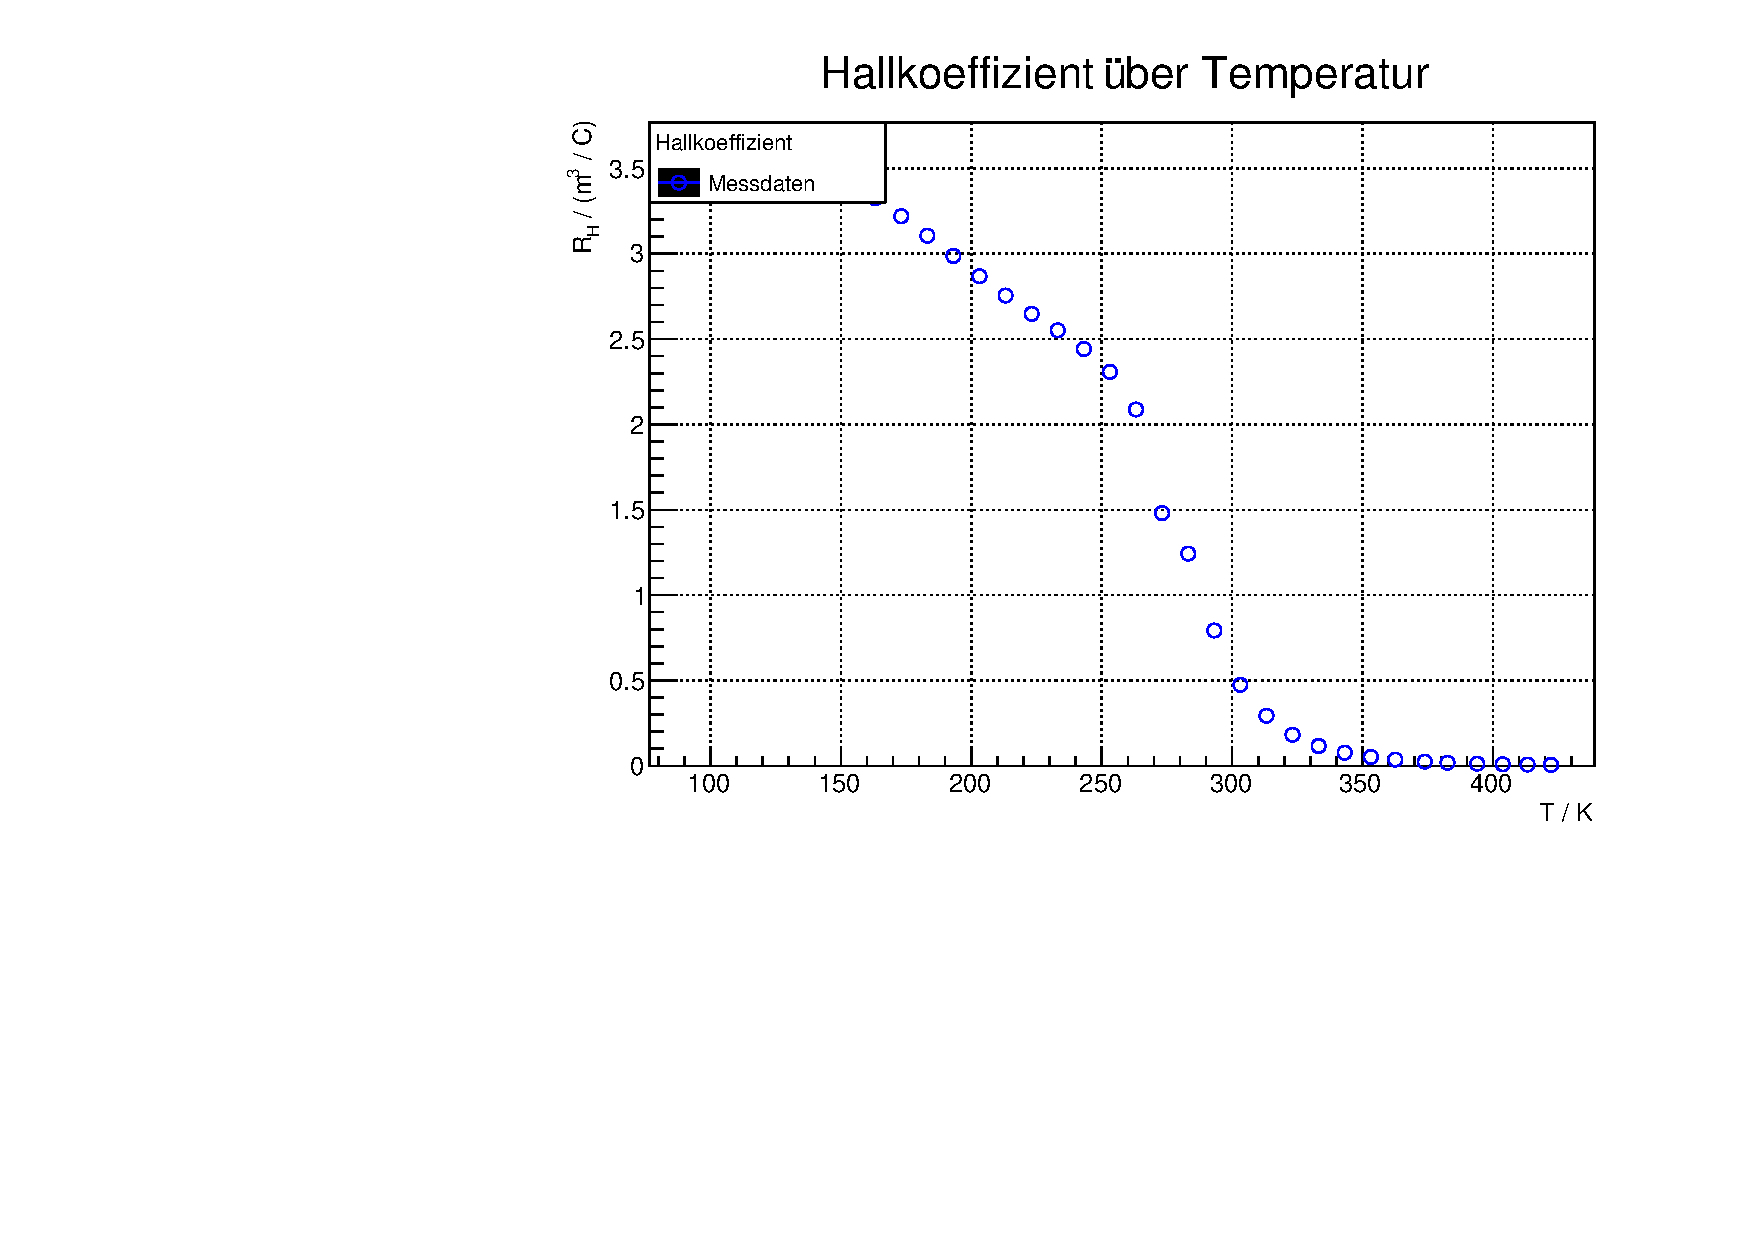
\includegraphics[scale = 0.5]{../data/A1R_h.pdf}
\caption{Hall Koeffizient von Probe A über der Temperatur}
\end{figure}

\begin{figure}
\label{fig:sigma}
\centering
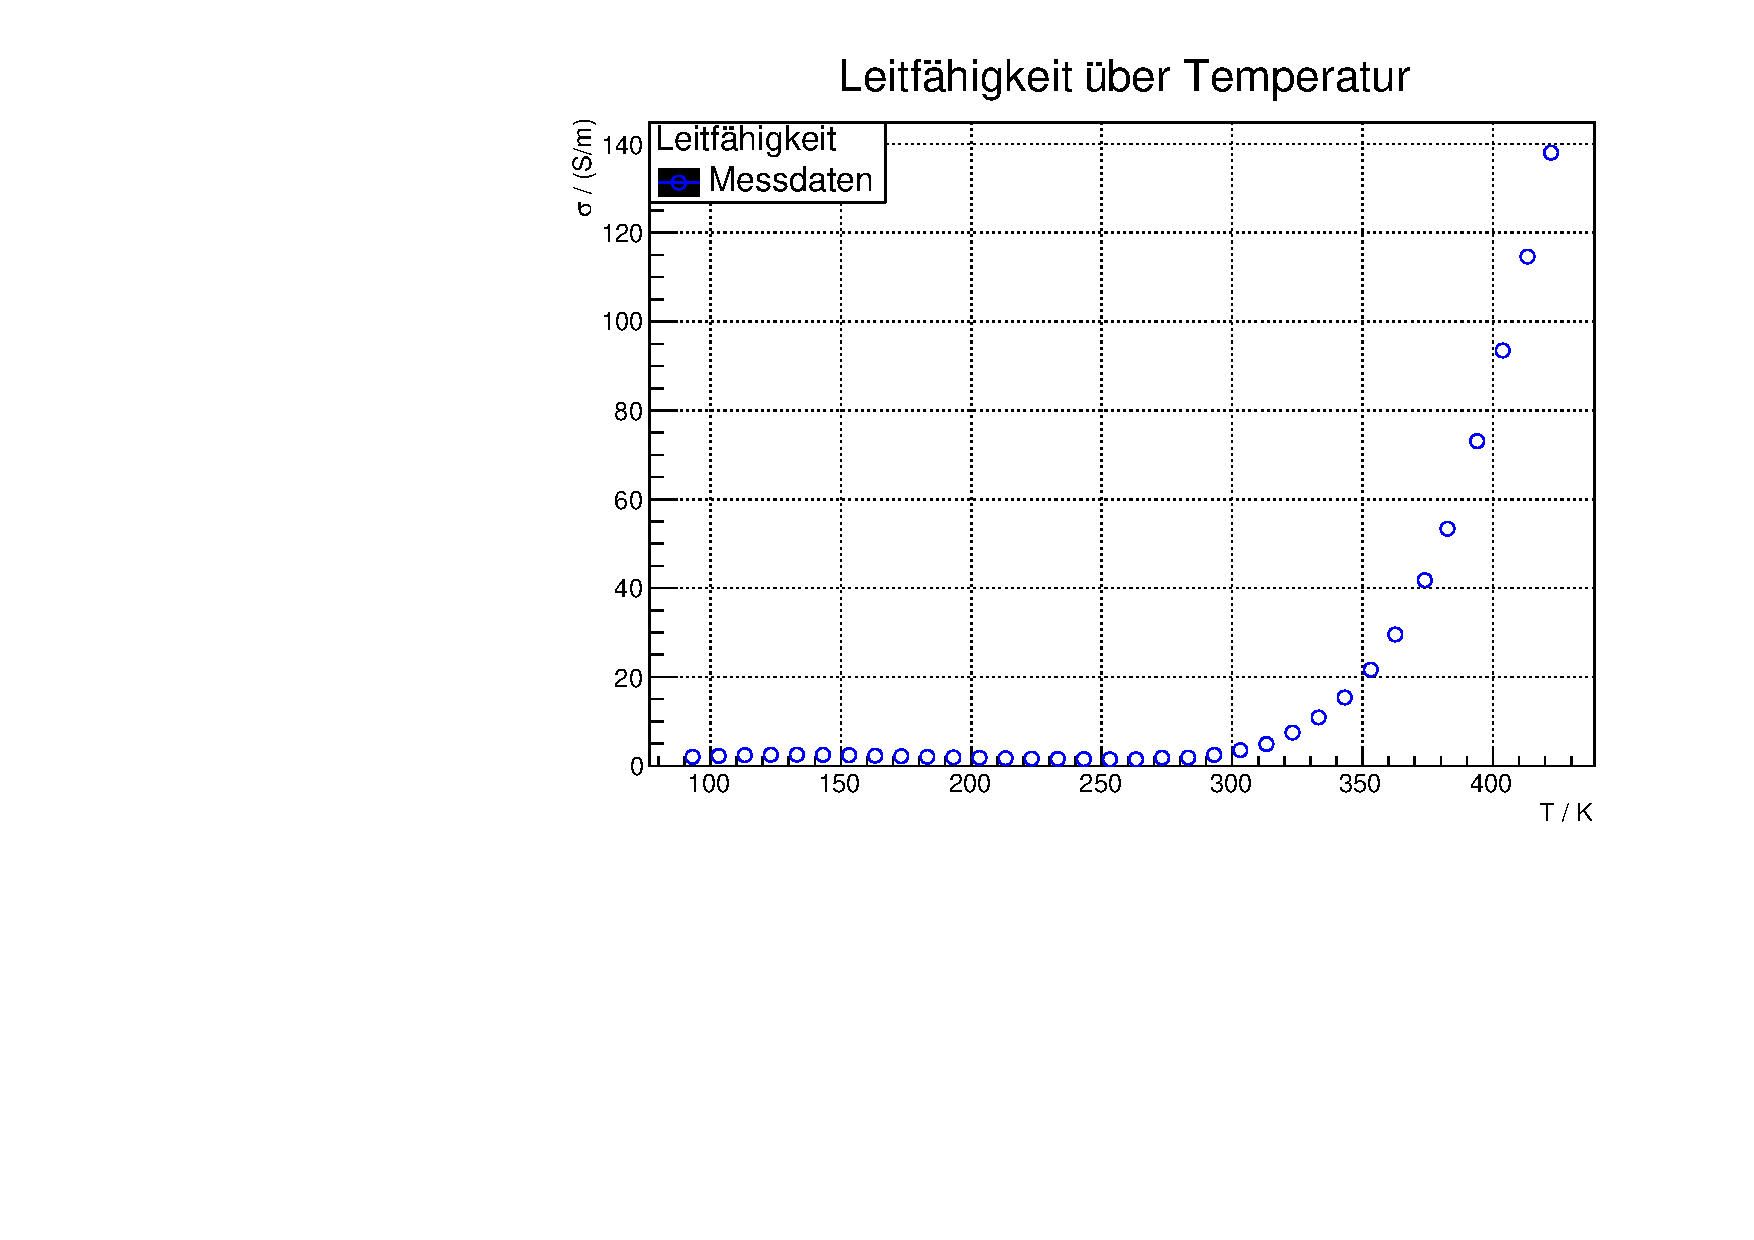
\includegraphics[scale = 0.5]{../data/A1sigma.pdf}
\caption{Leitfähigkeit von Probe A über der Temperatur}
\end{figure}


%formulas
%R_Hs = - UAH * b / (IAs * B ) * 0.001 # cubic meters / coulomb
%sigmas = l * IAs / (b * d * UAleit) # S / m # as should be

\FloatBarrier
\subsubsection{Leitungsbereiche}

Die Grenzetemperaturen für ex- und intrinsischen Leitungsbereich werden aus den Plots \ref{fig:leitex} und \ref{fig:leitin} abgelesen.
Der extrinsische Bereich endet mit dem Plateau im inversen Hallkoeffizienten bei 270K. Der intrinsische Bereich beginnt ab dem linearen Bereich in $\sigma \cdot R_{H}$ bei 310K.

%extrinsisch bis 270
%intrinsisch ab 310
\begin{figure}
\label{fig:leitex}
\centering
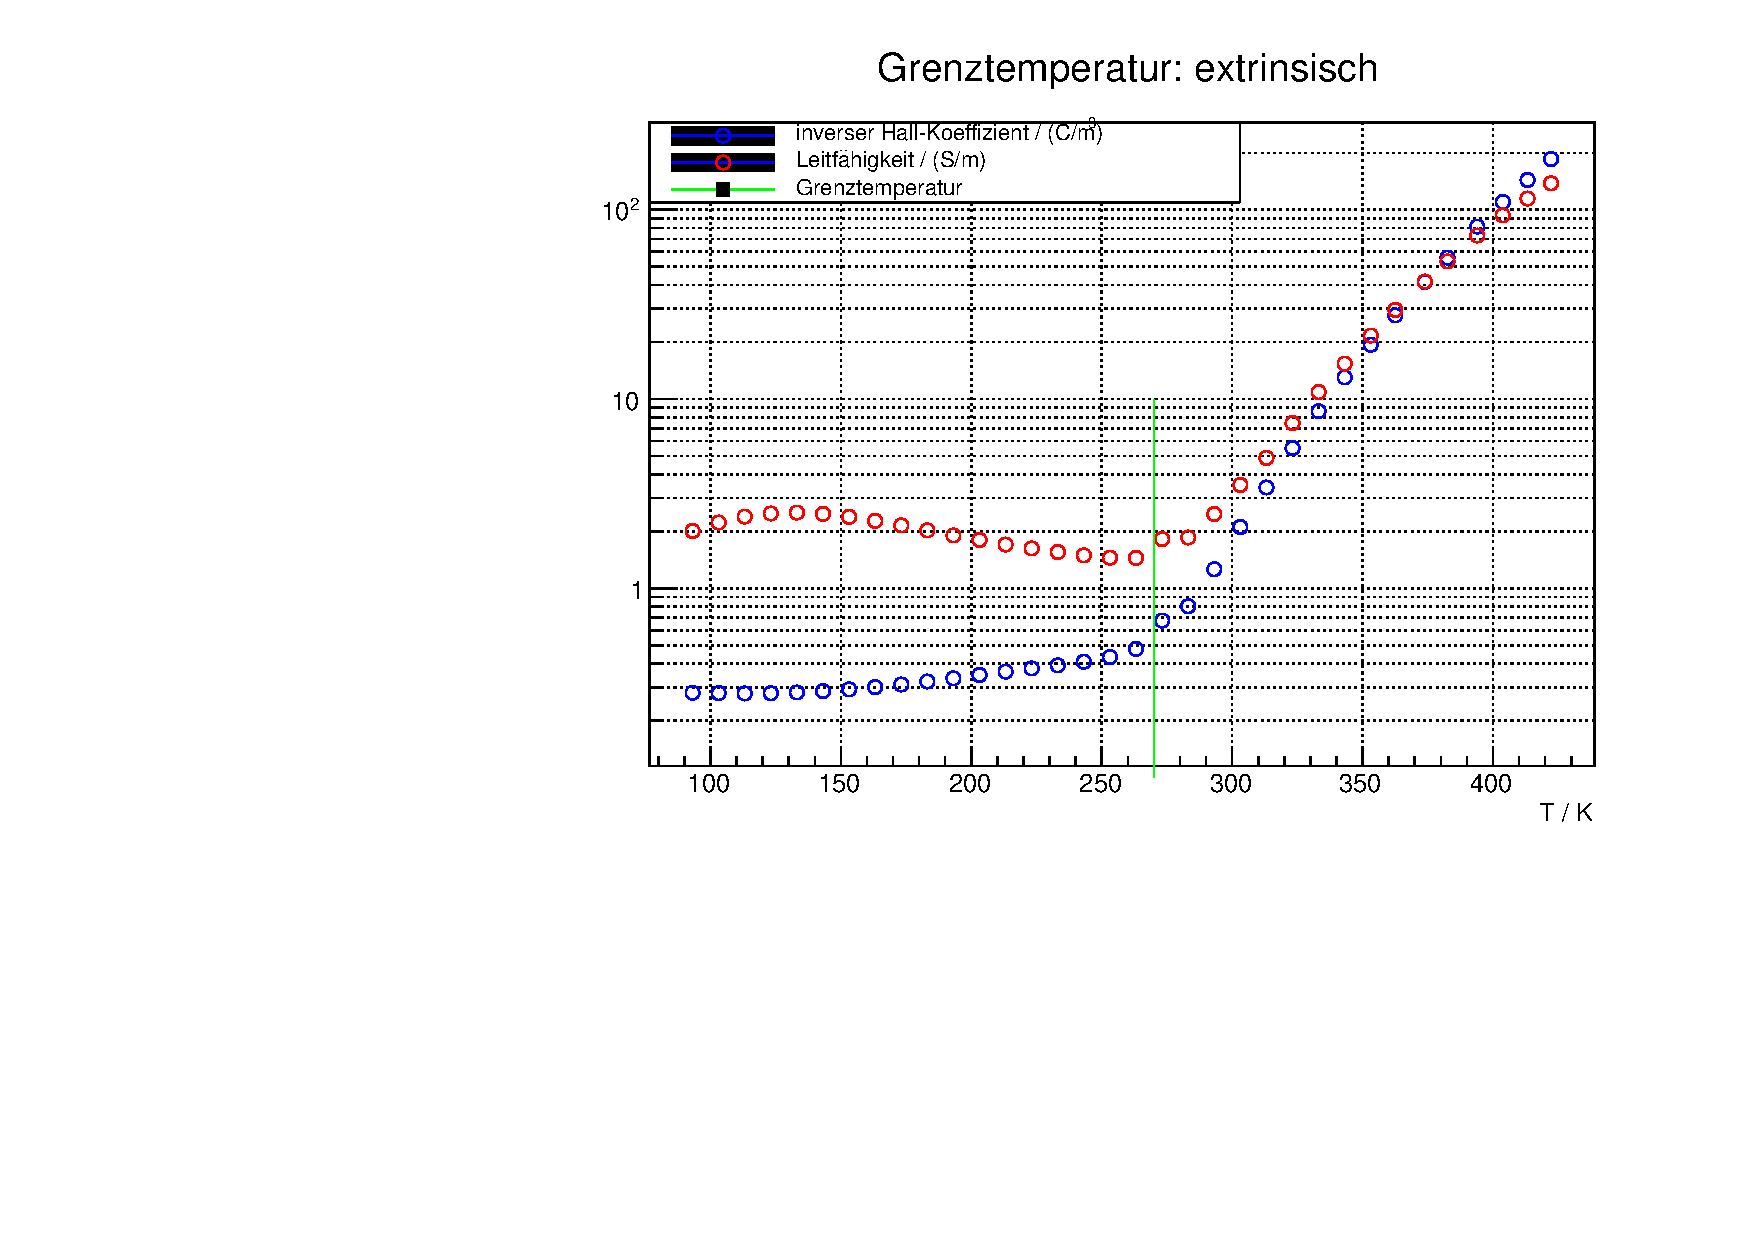
\includegraphics[scale = 0.35]{../data/A2ex.pdf}
\caption{Leitfähigkeit und inverser Hallkoeffizient}
\end{figure}

\begin{figure}
\label{fig:leitin}
\centering
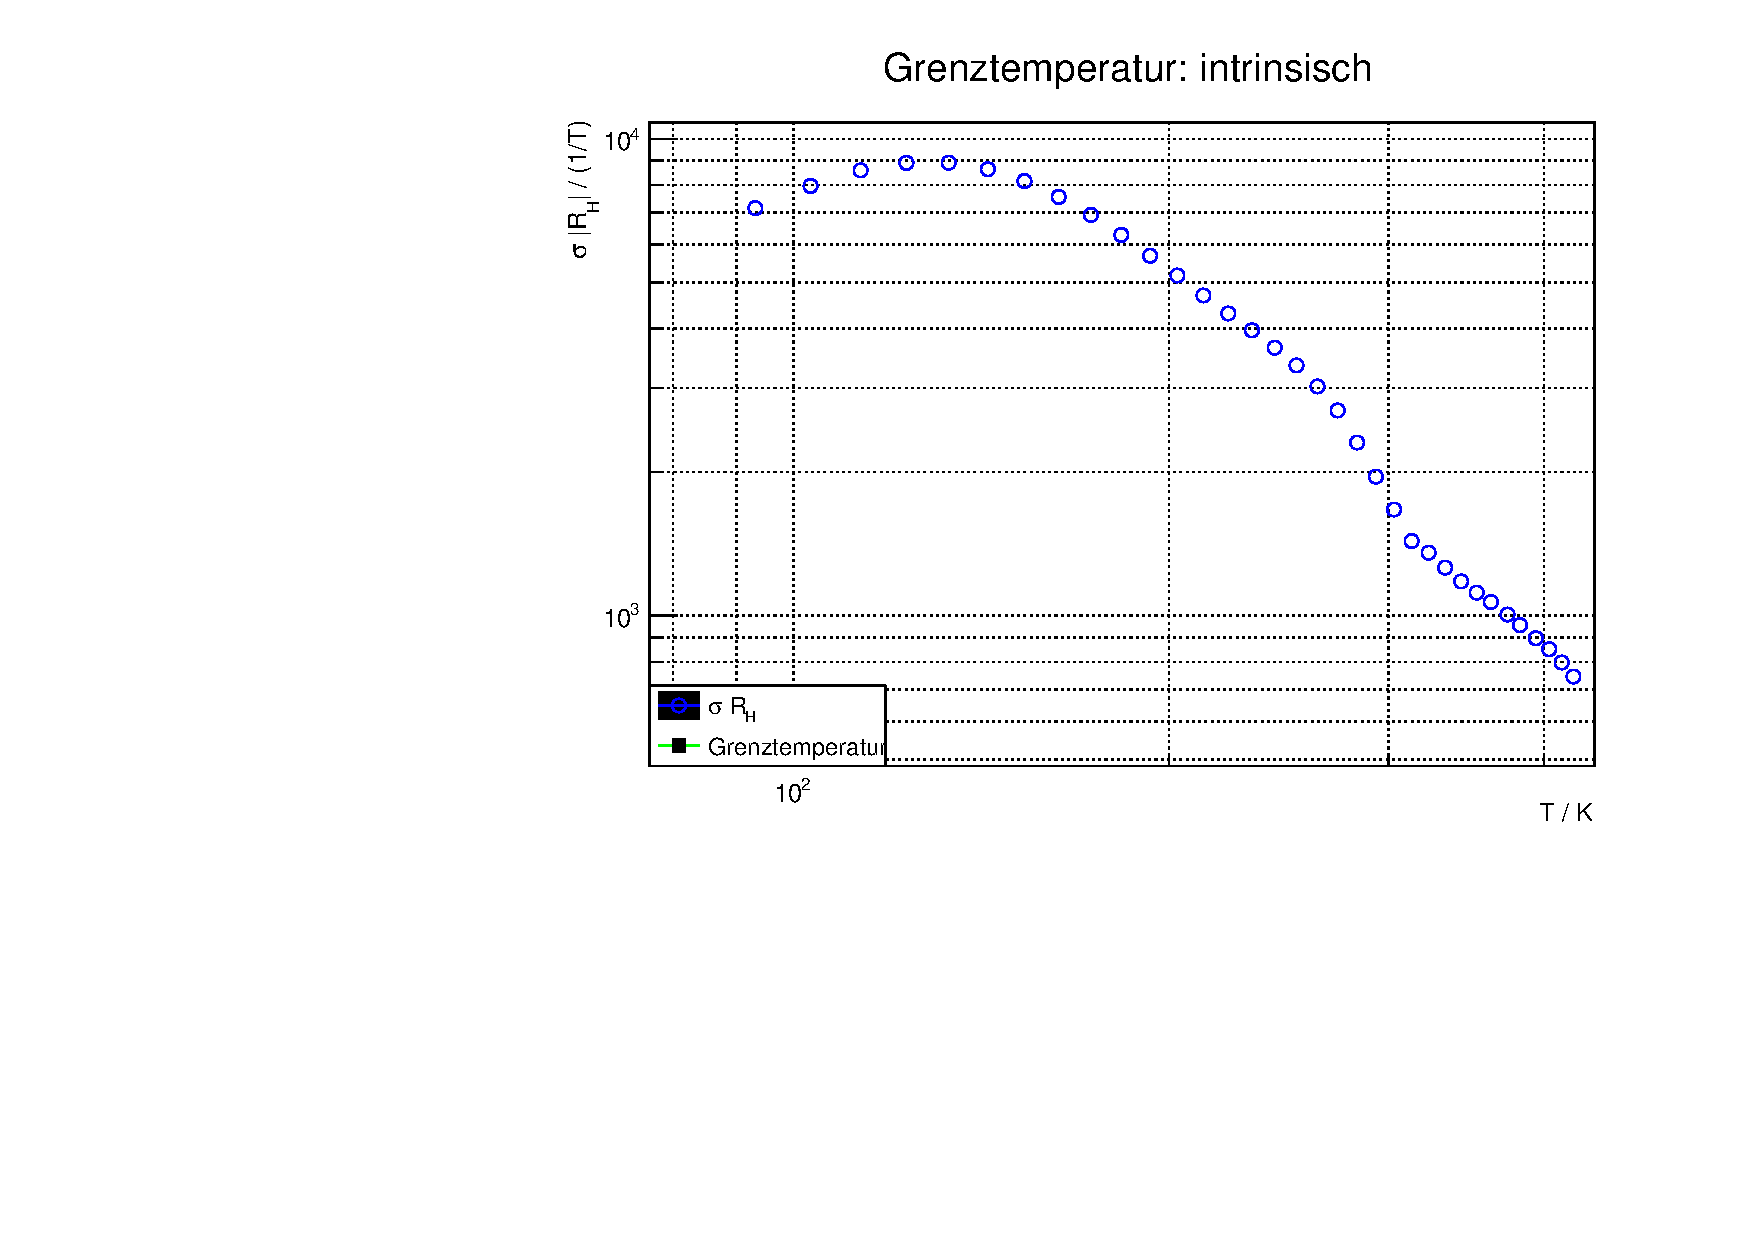
\includegraphics[scale = 0.35]{../data/A2in.pdf}
\caption{$\sigma \cdot R_{H}$}
\end{figure}

\FloatBarrier
\subsubsection{Leitungstyp}

Der Leitungstyp von Probe A kann aus dem Vorzeichen des Hallkoeffizienten abgelesen werden. Nach Vorbereitungsmappe Gl.51 gilt:
$$\vec{E}_H = - R_H (\vec{J} \times \vec{B}) $$
Somit ist das Vorzeichen der Hallspannung umgekehrt zu dem des Hallkoeffizienten. Weiter gilt für den Hallkoeffizienten
$$R_H = \frac{p\mu_p^{2} - n \mu _n ^{2}}{\vert e \vert (n \mu _n + p \mu _p)^{2}} $$
Da die Beweglichkeit für Elektronen größer ist, ist der Hallkoeffizient negativ im intrinsischen Fall, also für hohe Temperaturen. Liegt ein Vorzeichenwechsel mit steigender Temperatur vor so handelt es sich um Löcherleitung, da für tiefe Temperaturen der Koeffizient für Elektronleitung negativ und Löcherleitung positiv ist. \\
In unserem Fall sehen wir keinen Vorzeichenwechsel, woraus die bevorzugte Elektronleitung im extrinsischen Fall folgt. Der Halbleiter sollte also n-dotiert sein.
%Elektronenleitung???

\FloatBarrier
\subsubsection{Intrinsische Ladungsträgerkonzentration}
Die intrinsische Ladungsträgerkonzentration kann mit Hilfe von Formel (55) bestimmt werden. Die tabellierten Werte befinden sich im Anhang.

\begin{figure}
\label{fig:leitin}
\centering
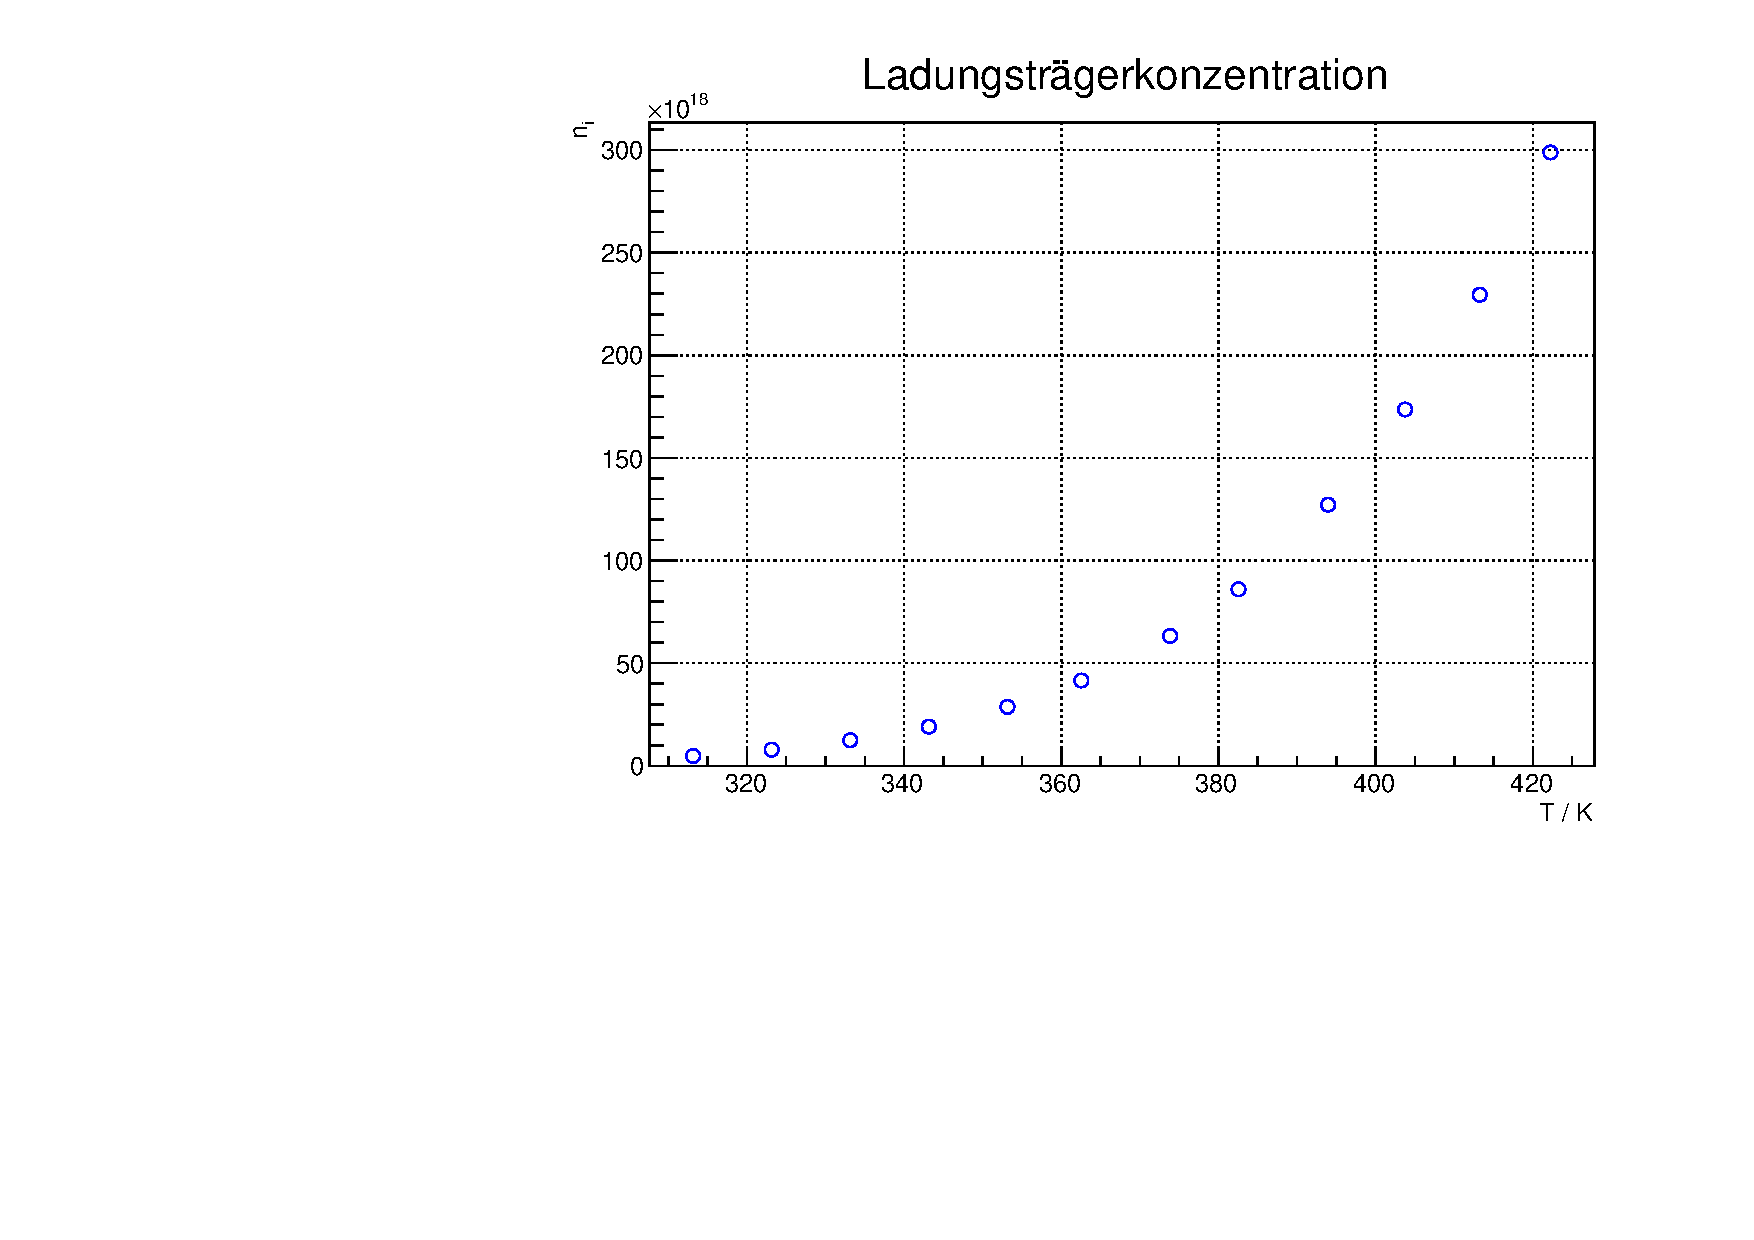
\includegraphics[scale = 0.5]{../data/A4.pdf}
\caption{Ladungsträgerkonzentration}
\end{figure}



\subsubsection{Arrhenius}
\FloatBarrier

%TODO oskar units
Aus dem Arrhenius-plot ergibt sich mit einem linearen Fit für die Bandlückenenergie und den y-Achsenabschnitt:
%$$y = -4467.87 \cdot x + 48.6613$$
$$\text{ln}(A) = 48.6613 \pm 0.0152968 $$
$$ - \frac{E_{G,0}}{2 \cdot k_B} = (-4467.87 \pm 5.55688 ) \ \text{K}$$
und damit:
$$E_{G,0} = 0.7695218869395287 \ \text{eV} $$

%y achsenabschnitt: 48.6613 +/- 0.0152968
%steigung: -4467.87 +/-5.55688
%E_G0 = -2 * kB * steigung
\begin{figure}
\label{fig:leitin}
\centering
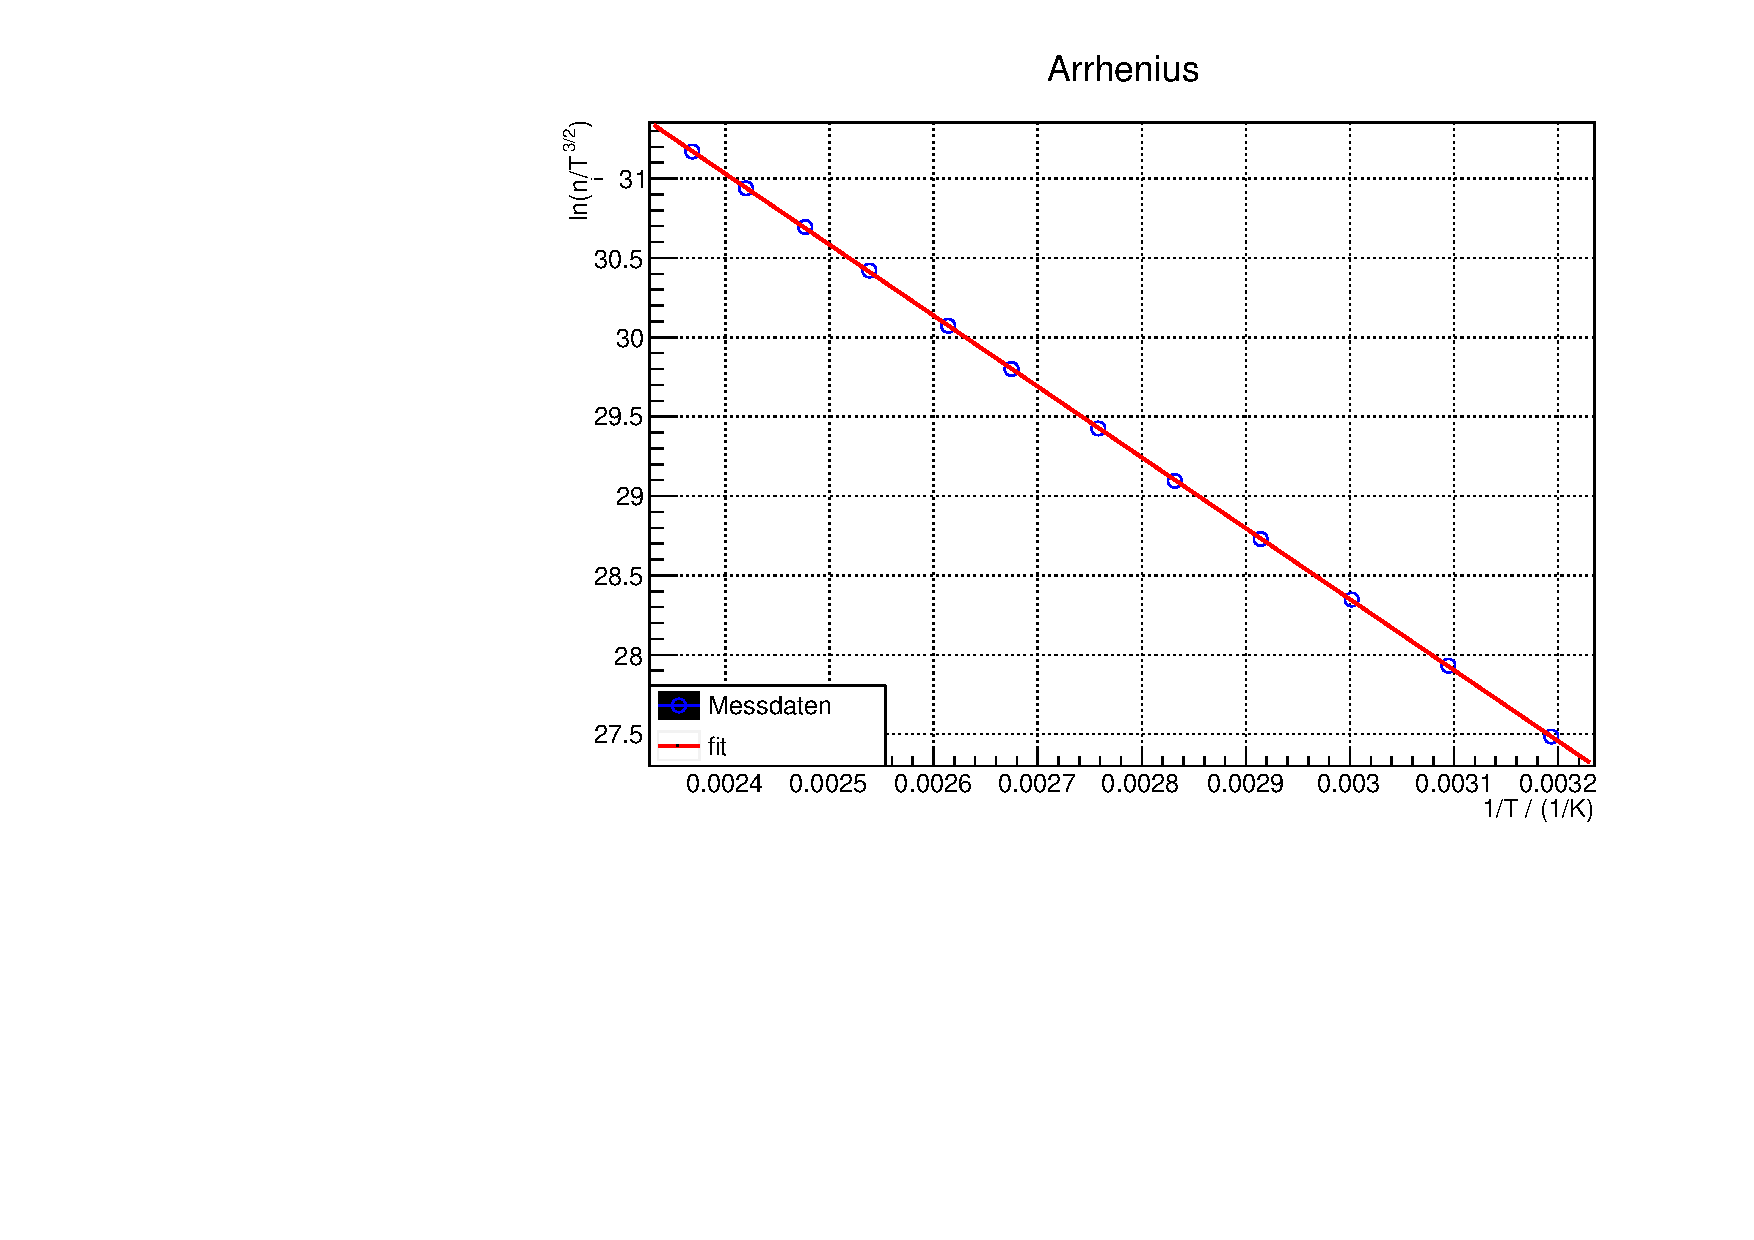
\includegraphics[scale = 0.5]{../data/A5.pdf}
\caption{Arrhenius plot}
\end{figure}


\subsubsection{Bandlücke bei 300K}
\FloatBarrier
Mit der Beziehung (44) aus der Vorbereitung gilt:
$$E_G(300K) = 0.6495218869395287 \ \text{eV}$$

\subsubsection{Intrinsische Ladungsträgerkonzentration bei 300K}
\FloatBarrier
Mit 
$$ n_i (T) = T^{3/2} \cdot A \cdot \exp^{- frac{E_{G,0}}{2 \cdot k_B }cdot T}$$
ergibt sich:
$$n_i(300) \text{K} = 2.4049587717810924E+18 \ m^{-3}$$

\subsection{Probe B}
\subsubsection{Beweglichkeit}
\FloatBarrier
Leitfähigkeit und Hall-Koeffizient für Probe B ergeben sich nach den angegebenen Formeln:
$$\sigma = \frac{\ln 2}{\pi} \frac{I}{U_{leit}}$$
$$R_H = \frac{U_H}{I} \frac{1}{B}$$
Die Tabelle für die Beweglichkeit befindet sich im Anhang.

\subsubsection{Vergleich: Volumenhalbleiter und 2DEG}
\FloatBarrier

Die Beweglichkeit für das 2DEG nimmt wie erwartet mit der Temperatur ab, da die Phononstreuung zunimmt. Im Volumenkristall nimmt die Beweglichkeit bei niedrigen Temperaturen zunächst zu, da die Störstellenstreuung mit der Temperatur abnimmt und dieser Effekt erst bei höheren Temperaturen durch die Phononstreuung kompensiert wird.

\begin{figure}
\label{fig:bbew}
\centering
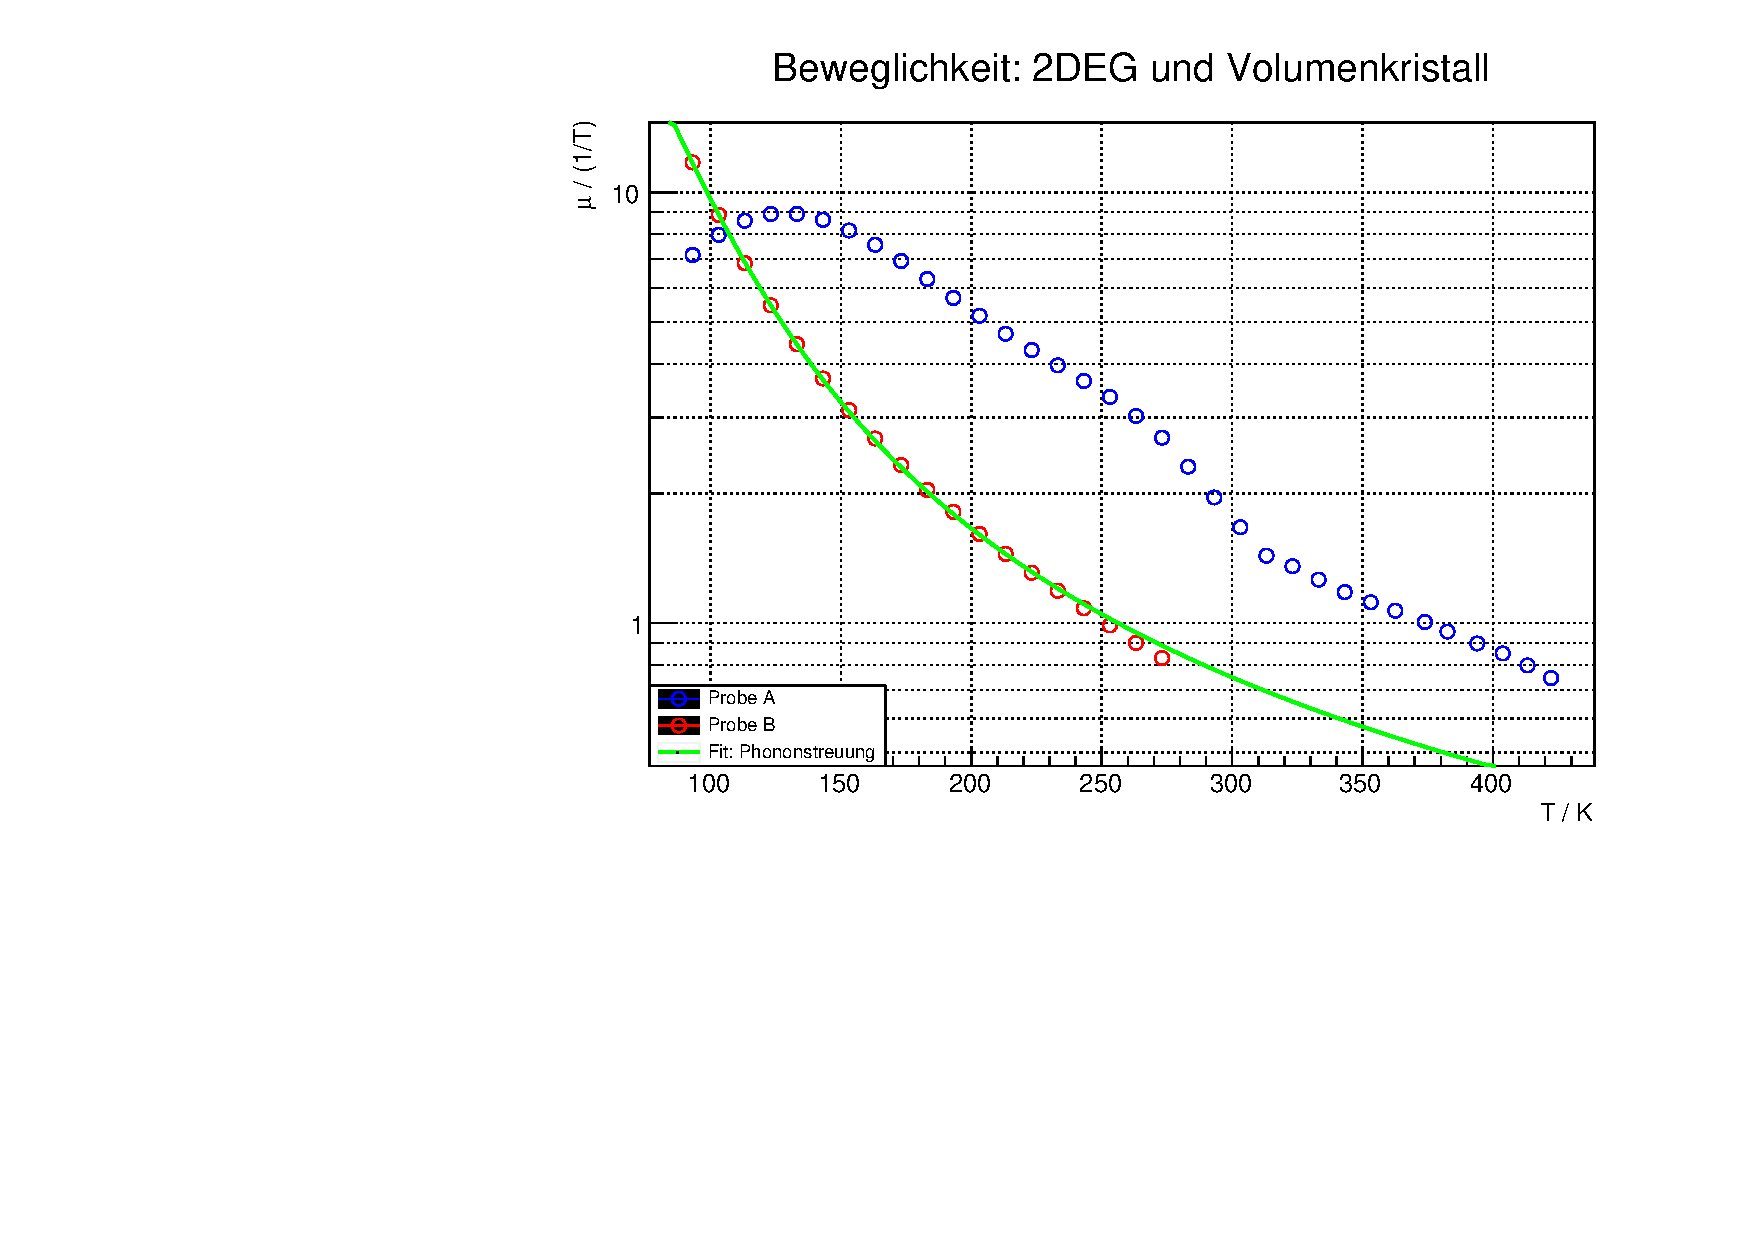
\includegraphics[scale = 0.5]{../data/B2.pdf}
\caption{Bewegleichkeiten für verschiedene Proben}
\end{figure}


%\subsection{Phononenstreuung}
%\FloatBarrier


